%===========================================================================================
%\section{History}
%===========================================================================================
%\subsection{Atomism}
%===========================================================================================
\section{The Standard Model}
According to the Standard Model (SM), all matter results from interactions between fundamental particles: lepton and quarks (fermions), and mediators (bosons).
Table \ref{tab:qrknlep} shows fermions of the standard model, their anti-particle equivalent would have all the signs reversed for the quantum numbers. For example, an anti-electron (\(e^+\)) and anti-electron-neutrino (\(\bar{\nu_e}\)) lepton number would flip to \((-1, 0, 0)\) and charges (\(Q\)s) would be \(+1\) and 0 respectively.

\begin{table}[htbp]
	\centering
	\begin{tabular}{c @{\hspace{5pt}} l |c|c|c|l|c|c|c|}
		% Top edges of both tables
		\cline{3-5} \cline{7-9}

		% Table Headers (overriding borders explicitly to ensure the outer walls exist)
		\multicolumn{2}{c|}{}              & \multicolumn{3}{c|}{Leptons} &              & \multicolumn{3}{c|}{Quarks}                                                                                         \\
		\cline{3-5} \cline{7-9}

		% Column Headers (merging the first two columns to center 'Category' with no borders)
		                                   &                              & \(l\)        & \(Q\)                       & \((L_e, L_\mu, L_\tau)\) &  & \(q\) & \(Q\)      & \((F_d, F_u, F_s, F_c, F_b, F_t)\) \\
		\cline{3-5} \cline{7-9}

		% Group A block
		\multirow{2}{*}{First generation}  & \ldelim\{{2}{*}              & \(e^-\)      & \(-1\)                      & (1, 0, 0)                &  & \(d\) & \(-1/3\)   & \((-1, 0, 0, 0, 0, 0)\)            \\
		                                   &                              & \(\nu_e\)    & 0                           & (1, 0, 0)                &  & \(u\) & \(2/3\)    & \((0, 1, 0, 0, 0, 0)\)             \\
		\cline{3-5} \cline{7-9}

		% Group B block
		\multirow{2}{*}{Second generation} & \ldelim\{{2}{*}              & \(\mu^-\)    & \(-1\)                      & (0, 1, 0)                &  & \(s\) & \( -1/3 \) & \((0, 0, -1, 0, 0, 0)\)            \\
		                                   &                              & \(\nu_\mu\)  & 0                           & (0, 1, 0)                &  & \(c\) & \(2/3\)    & \((0, 0, 0, 1, 0, 0)\)             \\
		\cline{3-5} \cline{7-9}

		% Group B block
		\multirow{2}{*}{Third generation}  & \ldelim\{{2}{*}              & \(\tau^-\)   & \(-1\)                      & (0, 0, 1)                &  & \(b\) & \(-1/3\)   & \((0, 0, 0, 0, -1, 0)\)            \\
		                                   &                              & \(\nu_\tau\) & 0                           & (0, 0, 1)                &  & \(t\) & \(2/3\)    & \((0, 0, 0, 0, 0, 1)\)             \\
		% Bottom edges of both tables                         
		\cline{3-5} \cline{7-9}
	\end{tabular}
	\label{tab:qrknlep}
	\caption{Three generations of leptons (left) and quarks (right).}
\end{table}
\begin{table}[htbp]
	\begin{tabular}{
		>{\centering\arraybackslash}m{2.8cm}
		>{\centering\arraybackslash}m{2.8cm}
		>{\centering\arraybackslash}m{2.8cm}
		>{\centering\arraybackslash}m{2.8cm}
		}

		% ROW 1: Strong Vertices
		\multicolumn{1}{c}{\vhead{Electromagnetic} }                                                      & \multicolumn{3}{l}{\vhead{Strong}} \\[0.1cm]
		\threevertex{fermion}{X^{+|-}}{fermion}{X^{-|+}}{photon}{\gamma}                                  &
		\threevertex{fermion}{q}{fermion}{q}{gluon}{g}                                                    &
		\threevertex{gluon}{g}{gluon}{g}{gluon}{g}                                                        &
		\fourvertex{gluon}{g}{gluon}{g}{gluon}{g}{gluon}{g}
		\\[1cm]

		% ROW 3: Electromagnetic and Electroweak Vertices
		\multicolumn{3}{l}{\vhead{Weak}}                                                                  &                                    \\[0.1cm]
		\threevertex{fermion}{\nu_e \mid \nu_\mu \mid \nu_\tau}{fermion}{e \mid \mu \mid \tau}{photon}{W} &
		\threevertex{fermion}{d/s/b}{fermion}{u/c/t}{photon}{W}                                           &
		\threevertex{fermion}{f}{fermion}{f}{photon}{Z}                                                   &



		\\[1cm]
		\multicolumn{2}{l}{\vhead{Electroweak}}                                                           & \multicolumn{2}{l}{\vhead{Higgs}}  \\[0.1cm]
		\threevertex{photon}{Z/\gamma}{photon}{W}{photon}{W}                                              &
		\fourvertex{photon}{W}{photon}{W}{photon}{W|Z/\gamma}{photon}{W|Z/\gamma}                         &
		\threevertex{fermion}{m}{fermion}{m}{scalar}{H}                                                   &
		\fourvertex{scalar}{H}{scalar}{H}{scalar}{m_B}{scalar}{m_B}
	\end{tabular}
	\caption{Feynman diagrams of various interaction vertices possible in the Standard Model}
	\label{tab:smvtx}
\end{table}

The mediators/bosons exchanged between the other fundamental particles give rise to the fundamental interactions: electromagnetism from the photon (\(\gamma\)), weak force from \(W^\pm\) and \(Z\) bosons, the gluon (\(g\)) for the strong force, and the Higgs boson (\(h\)) for imparting mass to the fundamental particles. Various interaction vertices possible in SM, that become the building blocks of all fundamental interactions are shown in \ref{tab:smvtx}. 

%===========================================================================================
\section{Quantum Chromodynamics}

%\subsection{Lagrangian and Feynman Rules}
\emph{Quantum Chromodynamics (QCD)} is the component of the SM which describes the strong interactions of quarks and gluons. The QCD Lagrangian can be expected as:
\begin{align}
	\mathcal{L}_\mathrm{QCD} = &\underbrace{\bar{q}^\alpha (i \gamma^\mu \partial_\mu\delta_{\alpha\beta} - g\gamma^\mu
	t^a_{\alpha\beta}A^a_\mu - m\delta_{\alpha\beta})q^\beta - \frac{1}{4} F^a_{\mu\nu}F_a^{\mu\nu}}_{\mathcal{L}_\mathrm{classical}}\notag\\ &\underbrace{- \frac{1}{2\lambda}(\partial^\mu A^a_\mu)^2}_{\mathcal{L}_\mathrm{gauge-fixing}}+ \underbrace{\bar{c}^\alpha\partial^\mu(\partial_\mu\delta_{\alpha\beta} + igT^a_{\alpha\beta}A^a_\mu)c^\beta}_{\mathcal{L}_\mathrm{ghost}}
\end{align}

\(\mathcal{L}_\mathrm{classical}\) is the classical Lagrangian density shows interaction of a quark field  \(q^\alpha\) with 3 color degrees of freedom interacting with gluon fields \(A^a_\mu\) with 8 color degrees of freedom. \(g\) and \(m\) are dimensionless and correspond to QCD coupling constant, and quark-mass respectively. \(F^a_{\mu\nu}\) are the gluon tensors defined as,
\begin{equation}
	F^a_{\mu\nu} = \partial_\mu A_\nu^a - \partial_\nu A_\mu^a - gf_{abc}A^b_\mu A^c_\nu.
	\label{eq:gluonFieldTensor}
\end{equation}

To properly define gluon propagators, we need to make a choice of gauge. The \(\mathcal{L}_\mathrm{gauge-fixing}\) parametrizes the class of covariant gauges with the gauge parameter $\lambda$. In non-Abelian theories, this gauge fixing term leads to creation of unphysical degrees of freedom, which are canceled out by \(\mathcal{L}_\mathrm{ghost}\) which contains complex, scalar fermion fields \(c^\alpha\). 

 The matrices \(t^a\) and  \(T^a\) are the fundamental and adjoint representations of \(\rm SU(3)\) in form of traceless \(3\times3\) and \(8\times8\) hermitian matrices satisfying:
\begin{align}
	[t^a, t^b] = if_{abc}t^c,~\tr(t^at^b) = \frac{1}{2}\delta^{ab} \notag\\
	[T^a, T^b] = if_{abc}T^c,~(T^{a})_{bc} = -if^{abc}.
\end{align}

Comparing with quantum electrodynamics (QED), where the photon field tensor lacks the last term of Eqn. \ref{eq:gluonFieldTensor} as it is an Abelian, \(U(1)\) gauge theory, we can explain the presence of three/four-gluon vertices and absence of such vertices for the photon in Table \ref{tab:smvtx}. The lagrangian can be used to formulate \emph{Feynman rules} for calculating amplitude contributions from various propagators and vertices, which are shown in Tab. \ref{tab:qcdrules}. 

\begin{table}[htbp]
	\centering
	\begin{tabular}{
		>{\centering\arraybackslash}m{4.0cm}
		>{\raggedright\arraybackslash}m{10.4cm}
		}
		% --- PROPAGATORS
		\propagator{gluon}{A,\alpha}{B,\beta}{p}   &
		\(\delta^{AB}\left[-g^{\alpha\beta} + (1-\lambda)\dfrac{p^{\alpha}p^{\beta}}{p^{2}+i\epsilon}\right]
		\dfrac{i}{p^{2}+i\epsilon}\)                                                             \\[0.4cm]

		\propagator{ghost}{A}{B}{p}                &
		\(\delta^{AB}\,\dfrac{i}{p^{2}+i\epsilon}\)                                              \\[0.4cm]

		\propagator{fermion}{a,i}{b,j}{p}          &
		\(\delta^{ab}\,\dfrac{i}{(\slashed{p}-m+i\epsilon)_{ji}}\)                               \\[0.6cm]

		% --- VERTICES
		\yvertex{gluon}{B,\beta}{q}{gluon}{A,\alpha}{p}{gluon}{C,\gamma}{r} &
		\(-g\,f^{ABC}\left[(p-q)^{\gamma}g^{\alpha\beta} + (q-r)^{\alpha}g^{\beta\gamma}
		+ (r-p)^{\beta}g^{\gamma\alpha}\right]\)

		\smallskip

		(all momenta incoming, \(p+q+r=0\))                                                      \\[0.4cm]

		\fourvertex{gluon}{A,\alpha}{gluon}{C,\gamma}{gluon}{B,\beta}{gluon}{D,\delta} &
		\(\begin{aligned}
			-ig^{2}f^{XAC}f^{XBD}\left[g^{\alpha\beta}g^{\gamma\delta} - g^{\alpha\delta}g^{\beta\gamma}\right] \\
			-ig^{2}f^{XAD}f^{XBC}\left[g^{\alpha\beta}g^{\gamma\delta} - g^{\alpha\gamma}g^{\beta\delta}\right] \\
			-ig^{2}f^{XAB}f^{XCD}\left[g^{\alpha\gamma}g^{\beta\delta} - g^{\alpha\delta}g^{\beta\gamma}\right]
		\end{aligned}\)                                                                          \\[0.4cm]

		\yvertex{gluon}{A,\alpha}{}{ghost}{B}{}{ghost}{C}{q} &
		\(g\,f^{ABC}q^{\alpha}\)                                                                 \\[0.4cm]

		\yvertex{gluon}{A,\alpha}{}{fermion}{b,i}{}{fermion}{c,j}{} &
		\(-ig\,(t^{A})_{cb}\,(\gamma^{\alpha})_{ji}\)
	\end{tabular}
	\caption{Feynman rules for QCD in a covariant gauge with gauge parameter \(\lambda\):
		the gluon, ghost and quark propagators, followed by the three- and four-gluon,
		ghost-gluon and quark-gluon vertices.}
	\label{tab:qcdrules}
\end{table}


\subsection{The Running Coupling}
\label{subsec:runningCoupling}
At an energy scale \(Q\), consider a dimensionless observable \(X\). Lets assume that \(Q\) is sufficiently high that the quark masses become negligible in comparison. To calculate \(X\) as a perturbation series in the QCD coupling \(\alpha_s = \frac{g^2}{4\pi}\) (analogous to the QED fine structure constant), we need to remove ultraviolet divergences through renormalization. Renormalization introduces another arbitrary energy scale $\mu$ where the divergences are subtracted.  In general, \(X\) would depend on the ratio \(Q^2/\mu^2\) and post-renormalization coupling $\alpha_s(\mu^2)$. However, any physical observable should be independent of $\mu$:
\begin{align}
	\mu^2\frac{d X(Q^2/\mu^2, \alpha_s(\mu^2))}{d\mu^2} &= \left[\mu^2\frac{\partial}{\partial\mu^2} +  \mu^2\frac{\partial\alpha_s(\mu^2)}{\partial\mu^2}\frac{\partial}{\partial\alpha_s}\right] X(Q^2/\mu^2, \alpha_s(\mu^2)) = 0 \notag\\
	\implies & \left[-\frac{\partial}{\partial t} + \beta(\alpha_s) \frac{\partial}{\partial\alpha_s}\right] X(e^t, \alpha_s) = 0.
	\label{eqn:renormX}
\end{align} 

Where, \(t = \ln{\frac{Q^2}{\mu^2}}\), \(\beta(\alpha_s) = \mu^2\frac{\partial\alpha_s}{\partial\mu^2}\), \(\alpha_s\equiv\alpha_s(\mu^2(t))\)
\begin{align}
	\beta(\alpha_s) &= -\frac{\partial\alpha_s}{\partial t}\notag\\
		\implies  t &=  \int^{\alpha_s(Q^2)}_{\alpha_s}\frac{d\alpha_s}{\beta(\alpha_s)}\notag\\
			\implies & \frac{\partial\alpha_s(Q^2)}{\partial t} = Q^2\frac{\partial \alpha_s}{\partial Q^2}  =  \beta(\alpha_s(Q^2)), \quad\frac{\partial\alpha_s(Q^2)}{\partial\alpha_s} = \frac{\beta(\alpha_s(Q^2))}{\beta(\alpha_s)}
					\label{eq:runningCouplingIntro}
\end{align}

Substituting in Eq. \ref{eqn:renormX}, we see that \(X(1, \alpha_s(Q^2))\) is a valid solution. Thus the scale dependence in \(X\) comes from the \emph{running coupling} \(\alpha_s(Q^2)\).  Perturbatively expanding \(\beta(\alpha_s)\), we can write the \emph{renormalization group equation} as,

\begin{align}
Q^2\frac{\partial \alpha_s}{\partial Q^2}  = -\alpha_s^2(Q^2)\left(\beta_0 + \beta_1\alpha_s(Q^2) + \mathcal{O}(\alpha_s^2(Q^2))\right)
\label{eq:RGEquation}
\end{align}

Where,
\begin{equation}
	\beta_0 = \frac{1}{(4\pi)^2}\left(11 - \frac{2}{3}N_f\right), \quad \beta_1 =  \frac{1}{(4\pi)^4}\left(102 - \frac{38}{3}N_f\right)
\end{equation}

\begin{figure}[!htbp]
	\centering
	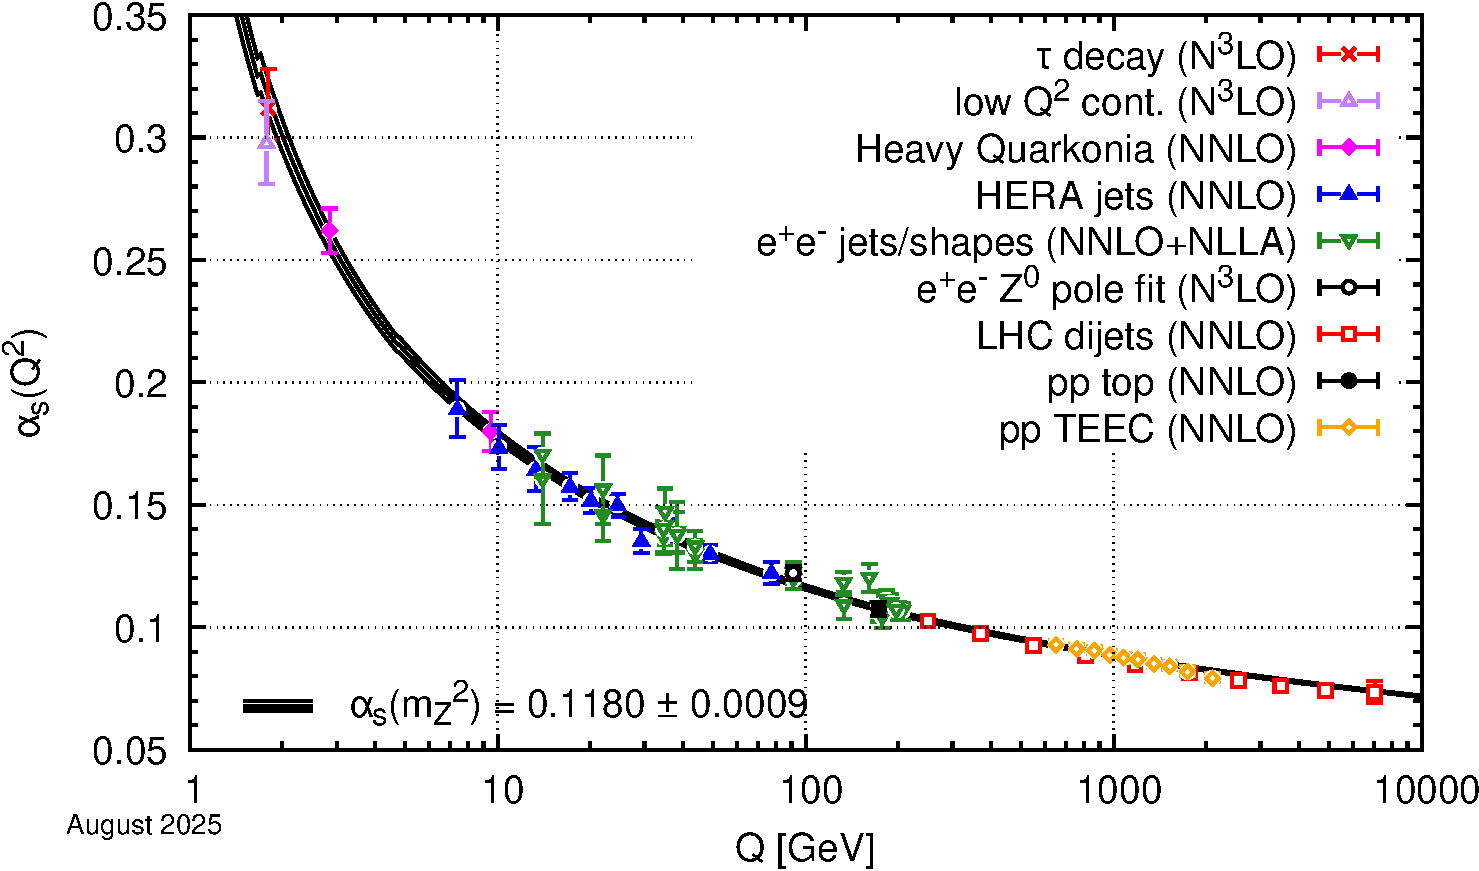
\includegraphics[width=0.7\linewidth]{figures/alphas-v-Q-2025-cropped.pdf}
	\caption{Summary of determinations of \(\alpha_s\) as a function of the energy scale Q compared to
		the running of the coupling computed at five loops taking as an input the current Particle Data Group (PDG) world average, \(\alpha_s(m_Z^2) = 0.1180 \pm 0.0009\) \cite{ParticleDataGroup:2026aaa}}
	\label{fig:runningCoupling}
\end{figure}

Integrating Eq. \ref{eq:RGEquation}
\begin{align}
	\ln(\frac{Q^2}{Q_0^2})  &= \int^{\alpha_s(Q^2)}_{\alpha_s(Q^2_0)}\frac{d\alpha_s}{\beta(\alpha_s)}\notag\\
	\implies \alpha_s(Q^2) &= \frac{\alpha_s(Q_0^2)}{1 + \beta_0(\alpha_s(Q_0^2))\ln(Q^2/Q_0^2) + \mathcal{O}(\alpha_s^2)}
	\label{eq:runningCouplingRel}
\end{align}

Usually, the reference scale \(Q_0^2\) is usually set to a convenient energy scale in the perturbative regime. \(\alpha_s\) at all other scales can be inferred accordingly. Usually, \(Q_0\) is set to mass of the \(Z\)-boson, \(m_Z\) as shown in Fig. \ref{fig:runningCoupling}. Another approach is to choose a scale parameter, \(\Lambda\) such that \(\alpha_s(\Lambda) \rightarrow \infty\).  

\begin{align}
	\ln(\frac{Q^2}{\Lambda^2}) &= - \int_{\alpha_s(Q^2)}^{\infty} \frac{d\alpha_s}{\beta(\alpha_s)}  \notag\\
	\implies \alpha_s(Q^2)  &= \frac{1}{\beta_0\ln(Q^2/\Lambda^2)}\left[1 - \frac{\beta_1}{\beta_0}\frac{\ln(\ln(Q^2/\Lambda^2))}{\ln(Q^2/\Lambda^2)} + \mathcal{O}\left(\frac{1}{\ln(Q^2/\Lambda^2)^2}\right)\right]
		\label{eq:runningCouplingLambda}
\end{align}

\(\Lambda\) is called the \emph{confinement scale}, around \(200~\mathrm{MeV}\). Eqs. \ref{eq:runningCouplingRel} and \ref{eq:runningCouplingLambda} show a monotonically decreasing relationship between \(\alpha_s\) and \(Q^2\). At high momentum transfers (\(Q \gg \Lambda\)), the coupling strength vanishes ($\alpha_s \to 0$). In this regime, quarks and gluons behave as quasi-free particles, making perturbative QCD (pQCD) calculations highly reliable (\emph{Asymptotic Freedom}).  At low energy scales (\(Q \ll \Lambda\)), the coupling diverges. In this non-perturbative QCD (npQCD) limit, isolated color charges cannot exist and partons are permanently bound into color-neutral hadrons (\emph{Color Confinement}).

\section{Hard Processes}
\subsection{Factorization}
To consider any nucleus as a singular coherent object, the fluctuations inside it would involve momentum transfers below the confinement scale (\(\Lambda\)) introduced in \ref{subsec:runningCoupling}, and would occur over timescales \(\sim 1/\Lambda\). We define \emph{hard-scattering processes} or just \emph{hard processes} as interactions of a hard perturbative probe with high momentum transfer \(Q >> \Lambda\). Since this interaction occurs over a time-scale \(\sim 1/Q \ll 1/\Lambda\), the perturbative probe effectively interacts with a near-static ``snapshot'' of the nucleus with a characteristic resolution \(\sim 1/Q\). 

\begin{figure}[htbp]
	\centering
	\factorizationdiagram
	\caption{Collinear factorization of a hadronic hard scattering.}
	\label{fig:factorization}
\end{figure}

Thus, we can \emph{factorize} the cross section of a collision process of nuclei with momentum \(P_1\) and \(P_2\) depicted by Fig. \ref{fig:factorization} as,

\begin{equation}
	\sigma(P_1, P_2)  = \sum_{i,j} \int dx_1dx_2f_i(x_1, \mu^2)f_j(x_2, \mu^2)\hat{\sigma}_{ij}(p_1, p_2, \alpha_s, Q^2/\mu^2)
	\label{eq:factorization}
\end{equation}

Where, the interactions occur between partons \(i\) from nucleus 1 and \(j\) from nucleus 2 carrying momentum \(p_1 = x_1P_1\) and \(p_2 = x_2P_2\) respectively. \(\mu\) is an arbitrary \emph{factorization scale}, often just set to \(Q\). The \(f_{k}(x, \mu^2)\) are the \emph{parton densities} giving likelihood of a parton \(k\) to carry \(x\) fraction of it's parent nucleus's momentum at a particular factorization scale \(\mu\). \(\hat{\sigma}_{ij}\)  is the \emph{parton cross-section} for scattering of partons \(i\) and \(j\). We can approximate it to the \((n+k)\) order in \(\alpha_s\) as, 

\begin{equation}
	\hat{\sigma}_{ij}(p_1, p_2, \alpha_s, Q^2/\mu^2) = \alpha_s^k \sum_{m=0}^{n}\hat{\sigma}_{ij}^{(m)} (p_1, p_2, Q^2/\mu^2)\alpha_s^m
\end{equation}

Different hard processes will have different leading powers \(k\). \(W\) production will have \(k=0\) whereas perturbative dijet production with two outgoing quarks will have \(k=2\). 

The parton densities \(f_i(x,\mu^2)\) in Eq.~\ref{eq:factorization} are not calculable in perturbation theory, but they are \emph{universal}: once measured in one process they may be used to predict any other. Requiring the physical cross section of Eq.~\ref{eq:factorization} to be independent of the arbitrary scale \(\mu\), exactly as for the coupling in Sec.~\ref{subsec:runningCoupling},
\begin{equation}
	\mu^2\frac{d}{d\mu^2}\,\sigma(P_1,P_2) = 0,
	\label{eq:pdfRGE}
\end{equation}
ties the \(\mu\)-dependence of the densities to that of \(\hat{\sigma}_{ij}\).

\section{From partons to jets}
Outgoing partons evolve from higher to lower momentum transfer scales (say, \(t\)). Initially their evolution are modeled using the pQCD mechanism called \emph{parton shower}. Eventually, say at an infra-red scale cut-off \(t_0\), pQCD calculations stop being valid and npQCD processes like hadronization dominate. QCD Monte-Carlo programs combining parton shower at \(t < t_0\) and hadronization process at \(t > t_0\)  are called \emph{QCD event generators}


\subsection{Parton branching}
\label{subsec:dglap}
\begin{figure}[h]
\centering
\label{fig:splitKinematics}
\begin{tikzpicture}[>=latex, line width=0.6pt,]
	\node[draw,circle, minimum size=1cm, inner sep=2pt] (rest) at (-1,0) {\(\mathcal{M}_\mathrm{n}\)};
	\coordinate (splitPoint) at (0.5, 0);
	\coordinate (continual) at (2,0);
	\coordinate (splitUp) at (2, 1);
	\coordinate (splitDown) at (2, -1);
	\draw (rest) to [edge label=a] (splitPoint);
	\path[draw, dash pattern=on 2pt off 3pt on 4pt off 4pt] (splitPoint) -- (continual);
	\path[draw] (splitPoint) to [edge label=b] (splitUp);
	\path[draw] (splitPoint)  to [edge label'=c] (splitDown);
	
	\pic[draw, "\(\theta_a\)",  ->, angle eccentricity=1.7] {angle = continual--splitPoint--splitUp};
	\pic[draw, "\(\theta_b\)",  <-, angle eccentricity=2.] {angle = splitDown--splitPoint--continual};
\end{tikzpicture}
\hspace{1cm}
\begin{tikzpicture}[>=latex, line width=0.6pt]
	%\node[draw,circle, minimum size=1cm, inner sep=2pt, pattern=north west lines] (rest) at (-1,0) { };
	\coordinate (incoming) at (-1, 0);
	\coordinate (splitPoint) at (0.5, 0);
	\coordinate (continual) at (2,0);
		\node[draw,circle, minimum size=1cm, inner sep=2pt] (rest) at (2,1) {\(\mathcal{M}_\mathrm{n}\)};
	\coordinate (splitDown) at (2, -1);
	\draw (incoming) to [edge label=a] (splitPoint);
	\path[draw, dash pattern=on 2pt off 3pt on 4pt off 4pt] (splitPoint) -- (continual);
	\path[draw] (splitPoint) to [edge label=b] (rest);
	\path[draw] (splitPoint)  to [edge label'=c] (splitDown);
	
	\pic[draw, "\(\theta_a\)",  ->, angle eccentricity=1.7] {angle = continual--splitPoint--splitUp};
	\pic[draw, "\(\theta_b\)",  <-, angle eccentricity=2.] {angle = splitDown--splitPoint--continual};
\end{tikzpicture}
\caption{Kinematics of timelike (left) vs spacelike (right) parton branching}
\end{figure}

Consider timelike splitting of a parton, \(a\to b+c\) shown in Fig. \ref{fig:splitKinematics}. Let's assume the partons are massless, and define the evolution scale (\(t\)) as, 
\begin{align}
	t &\equiv p_a^2 \gg p_b^2, p_c^2 \notag\\
	\implies t &\approx 2E_bE_c(1 - \cos(\theta))  \approx z(1-z)E_a^2\theta^2
\end{align}
Where, \(z = E_b/E_a = 1 - E_c/E_a\) and \(\theta = \theta_a + \theta_b\) is the opening angle.  The cross-section of a \(n\)-parton final state branching processes can be calculated by considering \(n\)-parton matrix element.
\begin{equation}
	\label{eq:nPartonXsec}
	d\sigma_n = \mathcal{F}|\mathcal{M}_n|^2d\mathbf{\Phi}_n
\end{equation}

Where \(\mathcal{F}\) is the initial-state flux factor and \(\mathbf{\Phi}_n\) is phase space of the \(n\)-parton final state. In the branching process the \(n\)-parton pre-split phase space volume element:

\begin{equation}
	d\mathbf{\Phi}_{n} = \ldots \frac{d^3\mathbf{p}_a}{2(2\pi)^3E_a}
\end{equation}

will be replaced by the \(n+1\)-parton phase space:

\begin{align}
	d\mathbf{\Phi}_{n+1} &= \ldots \frac{d^3\mathbf{p}_b}{2(2\pi)^3E_b} \frac{d^3\mathbf{p}_c}{2(2\pi)^3E_c} \notag\\
	&= d\mathbf{\Phi}_{n} \frac{1}{4(2\pi)^3}dtdzd\phi
\end{align}

and the \(n+1\)-parton matrix element can be calculated from the \(n\)-parton matrix element as,

\begin{equation}
	|\mathcal{M}_{n+1}\big|^2 \sim \frac{8\pi\alpha_s}{t}CF|\mathcal{M}_n|^2
\end{equation}

Substituting in Eq. \ref{eq:nPartonXsec} and integrating away the \(d\phi\), we get,

\begin{align}
	d\sigma_{n+1} &= d\sigma_n \frac{dt}{t}dz\frac{\alpha_s}{2\pi}\int\frac{d\phi}{2\pi}CF \notag\\
	&= d\sigma_n \frac{dt}{t}dz\frac{\alpha_s}{2\pi} \hat{P}_{ba}
\end{align}

Same equation would hold for the space-like case. To obtain the evolution equations, we can frame the evolution in terms of the change in parton distribution function \(f(x,t)\) when the evolution scale \(t\) goes from \(t\) to \(t+\delta t\).  ,

\begin{align}
	\delta f_i(x, t) &= \delta f_\mathrm{in} - \delta f_\mathrm{out} \notag\\
	&=\frac{\delta t}{t} \sum_j \int_{0}^{1} dz \frac{\alpha_s}{2\pi} \left[\frac{\hat{P}_{ij}(z)}{z}f_j(x/z, t) - \hat{P}_{ji}f_i(x,t)\right]
 \end{align}

Introducing the \emph{Sudakov form factor}, which gives the probability of a parton \(i\) evolving from scale \(t\) to a softer scale \(t_0\) without a resolvable emission,

\begin{align}
	\Delta_i(t) \equiv \exp(-\sum_j\int_{t_0}^{t} \frac{dt^\prime}{t^\prime}\int dz\frac{\alpha_s}{2\pi} \hat{P}_{ji}(z))
\end{align}

We get the familiar DGLAP-like evolution equations,

\begin{align}
	t\frac{\partial}{\partial t}\left(\frac{f_i}{\Delta_i}\right) = \frac{1}{\Delta_i}\sum_j \int \frac{dz}{z}\frac{\alpha_s}{2\pi}
\hat{P}_{ij}(z)f_j(x/z, t)\end{align}

\begin{table}[htbp]
	\centering
	\setlength{\tabcolsep}{6pt}
	\renewcommand{\arraystretch}{1.6}
	\begin{tabular}{
			>{\centering\arraybackslash}m{2cm}
			>{\centering\arraybackslash}m{4.0cm}
			>{\raggedright\arraybackslash}m{8cm}
		}
		\toprule
		Kernel (\(ij\)) & Diagram & \(\hat{P}_{ij}(z)\) \\
		\midrule
		\(qq\) & \splitvertex{fermion}{q}{}{fermion}{q}{z}{gluon}{g}{1-z} &
		\(\displaystyle C_F\left[\frac{1+z^2}{1-z}\right]\) \\
		\(gq\) & \splitvertex{fermion}{q}{}{gluon}{g}{z}{fermion}{q}{1-z} &
		\(\displaystyle C_F\,\frac{1+(1-z)^2}{z}\) \\
		\(qg\) & \splitvertex{gluon}{g}{}{fermion}{q}{z}{anti fermion}{\bar{q}}{1-z} &
		\(\displaystyle T_R\left[z^2 + (1-z)^2\right]\) \\
		\(gg\) & \splitvertex{gluon}{g}{}{gluon}{g}{z}{gluon}{g}{1-z} &
		\(\displaystyle C_A\left[\frac{z}{1-z} + \frac{1-z}{z} + z(1-z)\right] \)\\
		\bottomrule
	\end{tabular}
	\caption[Leading-order DGLAP splitting functions and their diagrams]{%
		The four leading-order collinear splittings entering the DGLAP evolution
		of Eq.~\ref{eq:dglap}. The daughter parton \(i\) carrying momentum
		fraction \(z\) is drawn on the upper leg, the recoiling parton \((1-z)\)
		on the lower. The plus prescription (Eq.~\ref{eq:plusPrescription}) and
		\(\delta(1-z)\) terms regularize the soft limit and enforce the momentum
		and flavor sum rules~\cite{Ellis_Stirling_Webber_1996}.}
	\label{tab:splitfns}
\end{table}

To deal with singularities corresponding to soft gluons at \(z\to 1\), we introduce an explicit infrared cut-off \(z < 1-\epsilon(t)\) .  Requiring the transverse momentum in timelike branching \(a\to bc\) to be positive, 
\begin{align}
	p_T^2 &= z(1-z)p_a^2 - (1-z)p_b^2 - zp_c^2 > 0 \notag\\
	\implies& z(1-z) > t_0/t \notag\\
	\implies&  z, 1-z > \epsilon(t) = \frac{1 - \sqrt{1-4t/t_0}}{2}\simeq t_0/t \notag\\
	\implies& t_0/t < z < 1 - t_0/t
\end{align} 



\subsection{Coherent branching}
So far, we have taken into account colinear enhancements to all pQCD orders. 


%\begin{equation}
%	P_{qq}(z)\xrightarrow{z\to1}\frac{2C_F}{(1-z)_+},\qquad
%	P_{gg}(z)\xrightarrow{z\to1}\frac{2C_A}{(1-z)_+},
%	\label{eq:splitSoft}
%\end{equation}
%
%In that soft limit the diagonal kernels reduce to Eq.~\ref{eq:splitSoft}, so
%the rate of soft-gluon emission is fixed by the color charge of the radiating
%parton, \(C_A\) for a gluon against \(C_F\) for a quark. The mean number of
%emissions in the cascade grows in proportion, approaching
%\begin{equation}
%	\frac{\langle n \rangle_g}{\langle n \rangle_q} \longrightarrow
%	\frac{C_A}{C_F} = \frac{9}{4}
%	\label{eq:multRatio}
%\end{equation}
%in the asymptotic limit, so a gluon-initiated jet fragments into more
%constituents than a quark-initiated jet of the same energy
%
%A parton in the final state evolves by the same kernels, now read as timelike
%branchings toward lower scales. The \emph{fragmentation functions}
%\(D_{h/i}(z,\mu^2)\), giving the probability that a parton \(i\) hadronizes
%into a hadron \(h\) with momentum fraction \(z\), obey
%\begin{equation}
%	\frac{\partial D_{h/i}(z,\mu^2)}{\partial \ln\mu^2} =
%	\sum_{j}\int_z^1 \frac{dz'}{z'}\;\frac{\alpha_s(\mu^2)}{2\pi}\,
%	P_{ji}(z')\,D_{h/j}\!\left(\frac{z}{z'},\mu^2\right).
%	\label{eq:fragDGLAP}
%\end{equation}
%
%
%\subsection{Parton showers and the Sudakov form factor}
%\label{subsec:partonShower}
%
%Equation~\ref{eq:collinearEmission} admits a probabilistic reading that
%underlies the Monte Carlo simulation of QCD radiation. The differential
%probability of a resolvable branching per unit evolution,
%\begin{equation}
%	d\mathcal{P}_i = \frac{d\mu^2}{\mu^2}\int dz\;
%	\frac{\alpha_s(\mu^2)}{2\pi}\, P_i(z),
%	\label{eq:emitProb}
%\end{equation}
%exponentiates into the survival probability that a parton \(i\) evolves from a
%hard scale \(\mu_1^2\) down to a softer scale \(\mu_2^2\) \emph{without} a
%resolvable emission, the \emph{Sudakov form factor},
%\begin{equation}
%	\Delta_i(\mu_1^2, \mu_2^2) = \exp\left[
%	-\int_{\mu_2^2}^{\mu_1^2}\frac{d\mu'^2}{\mu'^2}
%	\int dz\; \frac{\alpha_s(\mu'^2)}{2\pi}\, P_{i}(z)\right],
%	\label{eq:sudakov}
%\end{equation}
%where the \(z\) integral runs over the resolvable region fixed by an infrared
%cutoff. Iterating---drawing the next scale from \(\Delta_i\) and the momentum
%fraction from \(P_i(z)\)---generates a \emph{parton shower}: an ordered cascade
%of \(1\to 2\) branchings evolving a single hard parton toward the hadronization
%scale, resumming the leading collinear logarithms
%\(\alpha_s^n \ln^n(\mu_1^2/\mu_2^2)\) to all orders. By Eq.~\ref{eq:splitSoft}
%the gluon Sudakov falls faster, so \(g\)-initiated showers branch more
%profusely than \(q\)-initiated ones, a difference that propagates into the
%internal structure of the resulting jets.

\begin{figure}[h]
	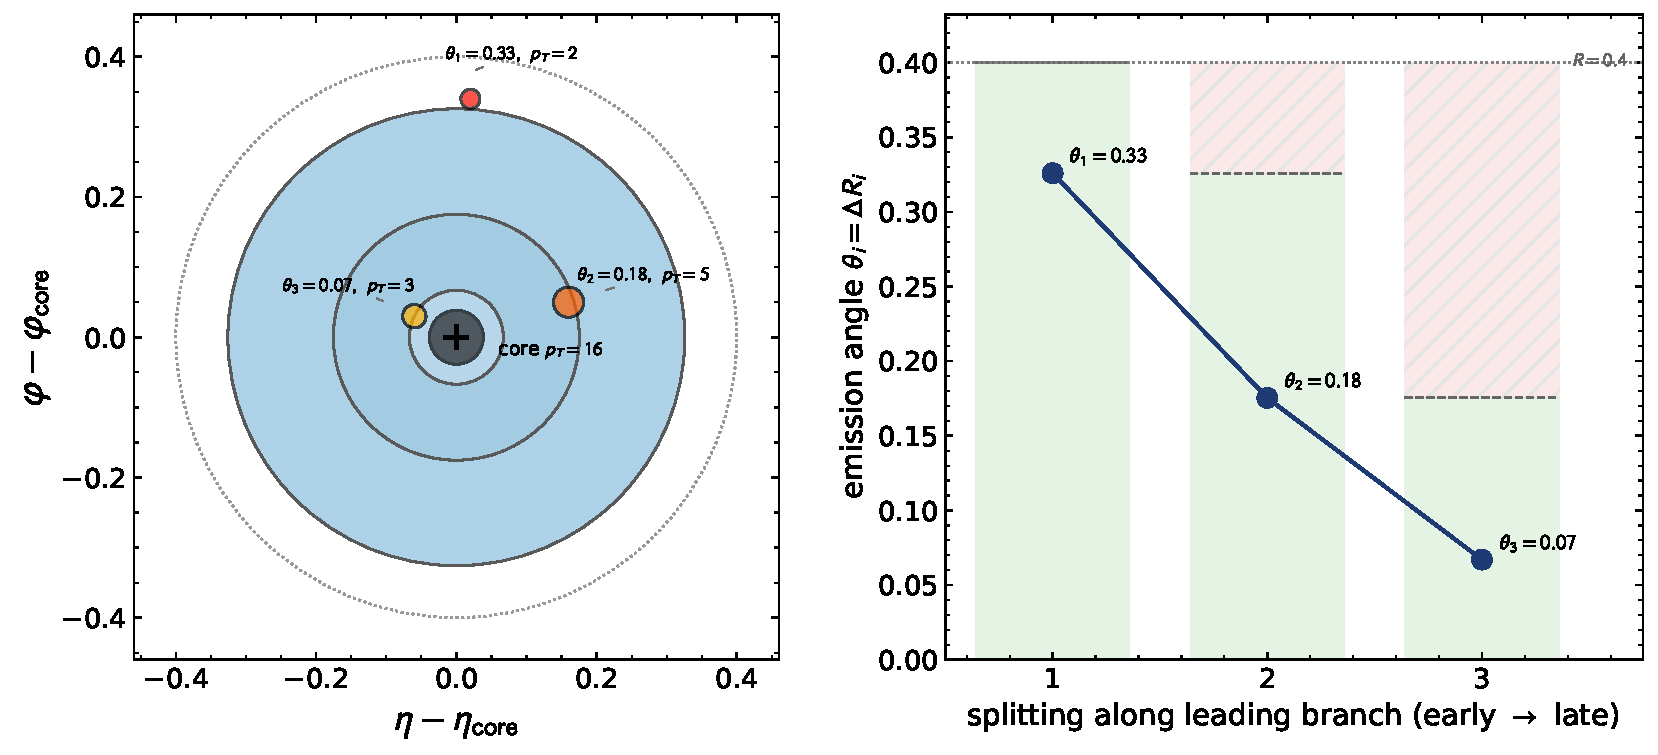
\includegraphics[width=\linewidth]{figures/fig_angular_ordering_cartoon.pdf}
\end{figure}

The ordering variable is not arbitrary. Quantum interference between
soft-gluon emissions---color coherence---suppresses large-angle radiation and
orders successive branchings in \emph{decreasing emission angle},
\begin{equation}
	\theta_1 > \theta_2 > \cdots > \theta_n .
	\label{eq:angularOrdering}
\end{equation}
This angular ordering imprints the color flow of the hard process onto the
angular distribution of radiation within the developing jet, and is the
microscopic origin of much of the substructure exploited in later chapters.

\subsection{Hadronization}
\label{subsec:hadronization}

The perturbative cascade terminates once emission scales approach \(\Lambda\),
where \(\alpha_s\) grows large (Sec.~\ref{subsec:runningCoupling}) and the
parton picture breaks down. The final conversion of colored partons into
color-neutral hadrons, \emph{hadronization}, is intrinsically non-perturbative
and is treated through phenomenological models tuned to data. In the Lund
string model \cite{lund} the color field between separating partons collapses
into a flux tube of constant tension, a linear confining potential
\begin{equation}
	V(r) = \kappa\, r,\qquad \kappa \approx 1~\mathrm{GeV/fm},
	\label{eq:stringPotential}
\end{equation}
whose breakup into hadrons is governed by the symmetric fragmentation
probability
\begin{equation}
	f(z) \propto \frac{1}{z}\,(1-z)^{a}\,
	\exp\!\left(-\frac{b\,m_T^2}{z}\right),
	\qquad m_T^2 = m^2 + p_T^2,
	\label{eq:lundFF}
\end{equation}
with tunable parameters \(a,b\). The net result is a collimated spray of
hadrons whose total energy and direction approximate those of the initiating
parton, and whose internal structure retains the imprint of the perturbative
evolution above. The reconstruction of these sprays as \emph{jets}, and the
observables built from their substructure, are the subject of the chapters
that follow.

\section{QCD phase diagram}
\begin{figure}[htbp]
	\centering
	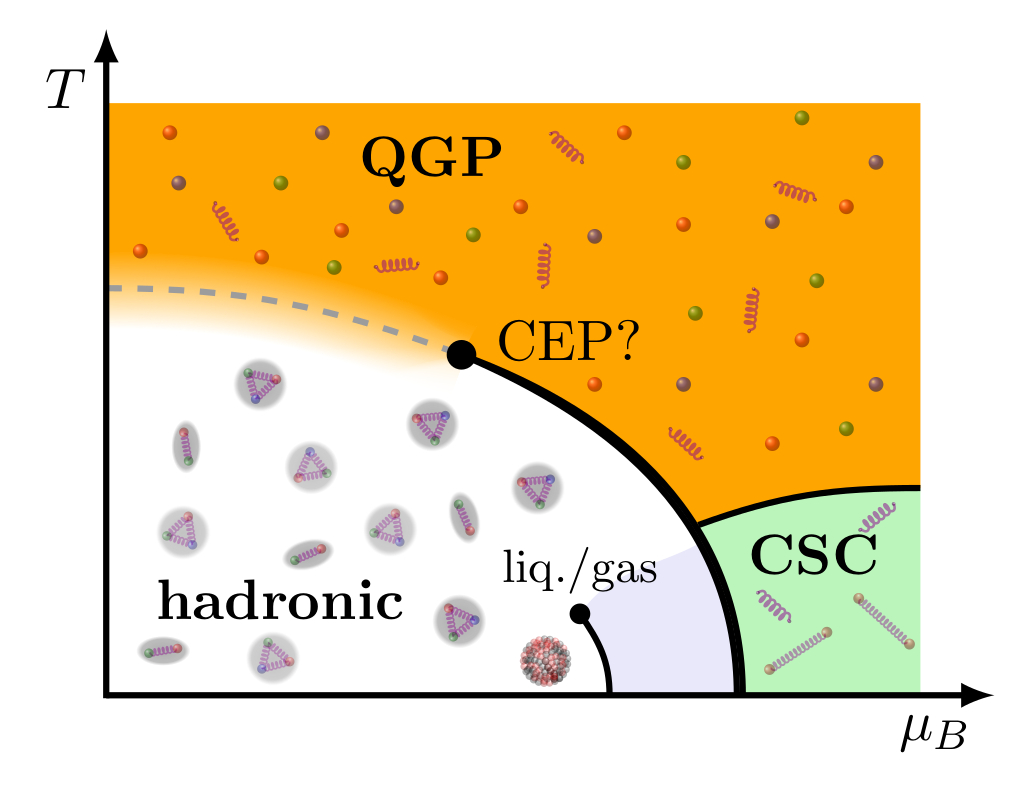
\includegraphics[scale=1]{figures/ownpd_mub_v2.jpg}
\end{figure}

\section{Event Generators}







%===========================================================================================


